\chapter{{\iqist}配置文件详解}
\label{chap:sci}

此前在第\ref{chap:inf}章的第\ref{sec:sci}节已经介绍了solver.ctqmc.in配置文件的标准格式,但是并没有解
释该文件所包含内容的具体含义。本章将详细描述solver.ctqmc.in配置文件中的各个控制参数。由于量
子杂质求解器组件仍在不断的更新,控制参数的具体定义与具体作用也在不断变化当中,因此本章的内容
仅仅作为用户的参考。关于各个控制参数的权威定义请参考相应量子杂质求解器的ctqmc\_control.f90文件以
及ctqmc\_stream.f90文件。

\section{isscf }
\label{sec:isscf}

{\color{red}含义}:控制量子杂质求解器组件的运行模式,该参数仅有如下两种可能的取值。
\begin{itemize}
\item isscf = 1,单步运行模式,量子杂质求解器仅仅被调用一次即中断。
\item isscf = 2,迭代运行模式,利用内置DMFT自洽条件反复调用量子杂质求解器进行迭代求解bethe晶格上的Hubbard模型。
\end{itemize}

{\color{green}类型}:integer

{\color{blue}缺省}:1

{\color{brown}组件}:全部

{\color{purple}注解}:isscf = 1此运行模式通常在LDA+DMFT计算中使用。此外,如果需要进行data binning或者是
精确计算观测量\footnote{例如精确计算自旋$-$自旋关联函数与虚时格林函数。}也可以应用此运行模式。在isscf = 1
运行模式下,用户通常需要提供正确的solver.hyb.in文件(参阅第\ref{sec:shi}节)与solver.eimp.in文件(参阅第\ref{sec:sei}节)。
如果用户不提供这两个文件,那么量子杂质求解器也能够正常运行,只是将会采用缺省的杂化函数并且将杂质轨道的能
级通通置为0。

\section{issun }
\label{sec:issun}

{\color{red}含义}:是否采用强制对称化,该参数仅有如下两种可能的取值。
\begin{itemize}
\item issun = 1, 不采用强制对称化。
\item issun = 2, 采用强制对称化,利用对称矢量所定义的对称性对各观测量进行对称化。
\end{itemize}

{\color{green}类型}:integer

{\color{blue}缺省}:1

{\color{brown}组件}:全部

{\color{purple}注解}:如果issun = 2,那么对称矢量symm(norbs)十分关键,它定义了不同轨道的对称性,亦即那些
轨道是简并的,那些轨道是不简并的。如果symm($i$) = symm($j$),那么认为第$i$条轨道与第$j$条轨道是简并的,
否则是非简并的。1 $\leq$ symm($i$) $\leq$ norbs。对称矢量可由文件solver.eimp.in中读入,缺省值为1。换言
之,如果在当前目录中不存在solver.eimp.in文件,并且issun = 2,那么量子杂质求解器组件将会认为所有轨道都是
简并的,并依此对物理观测量进行强制对称化。

如果您需要求解的量子杂质模型包含了自旋$-$轨道耦合项,那么我们强烈建议您采用如下配置:issun = 2, isspn = 2,
并且在solver.eimp.in文件中手动指定各个轨道之间的对称性。

如果您需要求解的量子杂质模型包含了磁性态,那么我们强烈建议您采用如下配置:issun = 2, isspn = 2,
并且在solver.eimp.in文件中手动指定各个轨道之间的对称性。

实际上,issun仅仅对$n_{\alpha}$,$G_{\alpha}(\tau)$,$\Delta_{\alpha}(\tau)$,$G_{\alpha}(i\omega)$与
$\Sigma_{\alpha}(i\omega)$等观测量有直接的影响,如果量子杂质求解器是迭代执行的,那么其余的观测量也会相
应地受到影响。

关于solver.eimp.in文件的细节,请参阅第\ref{sec:sei}节。

\section{isspn }
\label{sec:isspn}

{\color{red}含义}:是否对自旋自由度进行强制对称化,该参数仅有如下两种可能的取值。
\begin{itemize}
\item isspn = 1, 非磁或者是顺磁计算,自旋朝上的物理量与自旋朝下的物理量之间强制进行对称化。
\item isspn = 2, 铁磁或者是反铁磁计算,自旋朝上的物理量与自旋朝下的物理量之间不简并。
\end{itemize}

{\color{green}类型}:integer

{\color{blue}缺省}:1

{\color{brown}组件}:全部

{\color{purple}注解}:此控制参数通常与issun联用。从原则上说,isspn可以恒定为2,令issun = 2,并且通过
设定合适的symm(norbs)(通过solver.eimp.in文件),也可以对自旋自由度进行强制对称化。

isspn与issun是两个独立的控制参量,量子杂质求解器首先依据issun的取值决定是否进行轨道对称化,然后再根
据isspn的取值决定是否进行自旋对称化。前一种对称操作可能会被后一种对称操作所覆盖。例如考虑单带Hubbard
模型,如果issun = 2, 在solver.eimp.in文件中指定symm(1) = 1, symm(2) = 2,或者直接设定issun = 1,那么程序
将不会对轨道1和轨道2进行对称化。接下来考虑isspn,如果isspn = 2,那么同样不进行自旋对称化,轨道1与轨
道2之间不简并。如果isspn = 1,那么将会在轨道1和轨道2之间进行对称化。

如果您需要求解的量子杂质模型包含了自旋$-$轨道耦合项,或者是包含了磁性态,那么isspn必须设为2,否则计算结
果是不准确的。

\section{isbin }
\label{sec:isbin}

{\color{red}含义}:是否进入到data binning模式,该参数仅有如下两种可能的取值。
\begin{itemize}
\item isbin = 1, 正常计算模式。
\item isbin = 2, data binning模式。
\end{itemize}

{\color{green}类型}:integer

{\color{blue}缺省}:1

{\color{brown}组件}:全部

{\color{purple}注解}:当量子杂质求解器组件进入到data binning模式时,迭代数(iter)会固定为999,nsweep以及
nwrite会自动变为输入值的10倍,虚时格林函数被周期性输出到solver.green.bin.X文件中,其中X代表data bin的编
号,从1至nsweep/nwrite,后处理程序\footnote{例如{\hibiscus}组件中的maketau程序,请参阅
第\ref{sec:hib-tool}节。}将利用这些data bins对虚
时格林函数进行解析延拓。

isbin与isscf组合,将可以得到如下四种不同的运行模式:

\begin{itemize}
\item A: isscf = 1, isbin = 1,量子杂质求解器组件执行一次,不涉及DMFT自
洽迭代,采用正常计算模式,不进行data binning。
\item B: isscf = 2, isbin = 1,量子杂质求解器组件执行多次,利用DMFT方程
进行自洽迭代,在迭代过程中采用正常计算模式,迭代完毕后即停止,不进行data binning。
\item C: isscf = 1, isbin = 2,量子杂质求解器组件执行一次,不涉及DMFT自
洽迭代,直接进入到data binning模式。
\item D: isscf = 2, isbin = 2,量子杂质求解器组件执行多次,利用DMFT方程
进行自洽迭代,在迭代过程中采用正常计算模式,在迭代完毕后,量子杂质求解
器组件进入到data binning模式中执行一次。
\end{itemize}

\begin{figure}
\centering
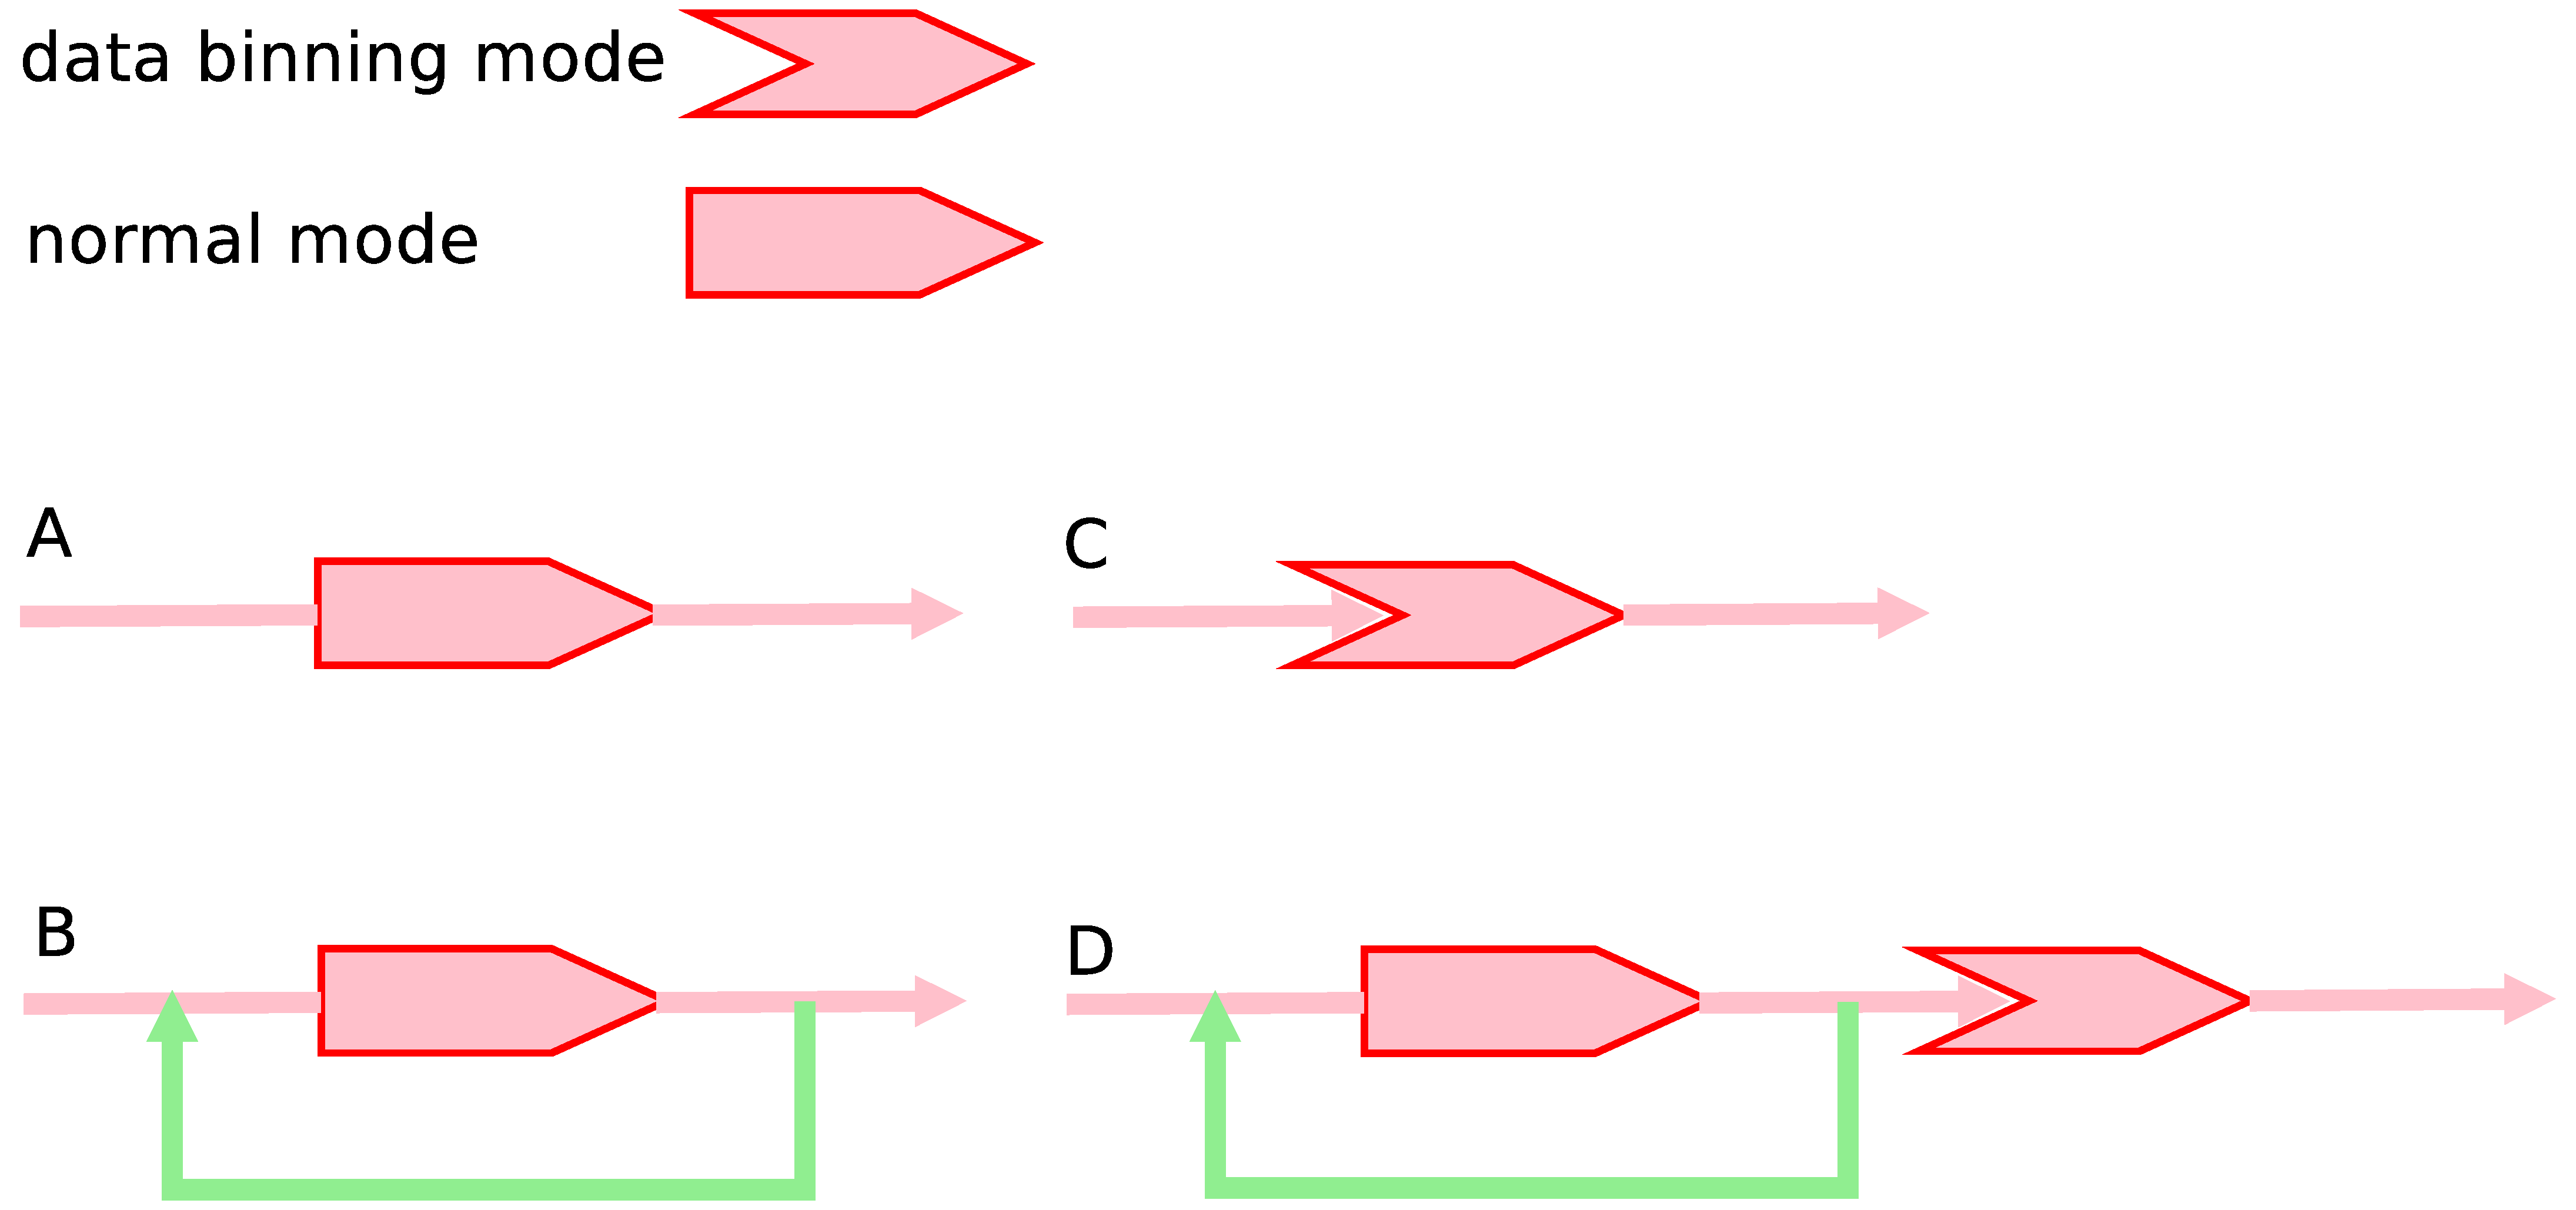
\includegraphics[scale=0.20]{figure/flow.eps}
\caption{量子杂质模型求解器组件的四种运行模式} 
\label{fig:flow}
\end{figure}

关于上述四种运行模式的解释可以参考图\ref{fig:flow}。如果用户需要进行
LDA + DMFT计算,那么可以利用运行模式A。模式B通常用于迭代求解一般的模
型哈密顿量,粗略判断计算结果是否合理。如果用户已经迭代求解DMFT方程完毕,需
要获得更为精确的结果,或者是为后处理步骤准备必须的数据,那么可以利用
运行模式C。运行模式D则相当于模式B与模式C的组合,一般很少使用。

\section{isort }
\label{sec:isort}

{\color{red}含义}: 是否应用正交多项式模式改善物理量的测量精度,该参
数仅有如下六种可能的取值。
\begin{itemize}
\item isort = 1,采用正常方法测量$G(\tau)$。
\item isort = 2, 采用Legendre正交多项式方法测量$G(\tau)$。
\item isort = 3,采用Chebyshev正交多项式方法测量$G(\tau)$。
\item isort = 4,采用正常方法测量$G(\tau)$与$F(\tau)$。
\item isort = 5,采用Legendre正交多项式方法测量$G(\tau)$与$F(\tau)$。
\item isort = 6,采用Chebyshev正交多项式方法测量$G(\tau)$与$F(\tau)$。
\end{itemize}

$G(\tau)$为虚时杂质格林函数,$F(\tau)$为附加关联函数,利用它可以解析地计
算出$\Sigma(i\omega)$,提高自洽计算的稳定性与可靠性。

{\color{green}类型}:integer

{\color{blue}缺省}:1

{\color{brown}组件}:仅{\gardenia}、{\narcissus}、{\lavender}组件

{\color{purple}注解}:{\gardenia}与{\narcissus}组件支持isort = $1 \sim 6$,但是{\lavender}
组件仅仅支持isort = $1 \sim 3$。

当isort = 1时,采用正常方法测量$G(\tau)$与$G(i\omega)$的低频部分。然后
在ctqmc\_make\_hub1()子程序中,利用Dyson方程计算低频部分的自能函数
$\Sigma(i\omega)$,将其与高频部分的原子自能函数
$\Sigma_{\text{atom}}(i\omega)$拼接起来,最后再利用Dyson方程计算最终的$G(i\omega)$。

当isort = 2时,采用Legendre正交多项式方法测量$G(\tau)$,采用正常方法测
量$G(i\omega)$的低频部分。然后在ctqmc\_make\_hub1()子程序中,利用
Dyson方程计算低频部分的自能函数$\Sigma(i\omega)$,将其与高频部分的原
子自能函数$\Sigma_{\text{atom}}(i\omega)$拼接起来,最后再利用Dyson方
程计算最终的$G(i\omega)$。

当isort = 3时,采用Chebyshev正交多项式方法测量$G(\tau)$,采用正常方法测
量$G(i\omega)$的低频部分。然后在ctqmc\_make\_hub1()子程序中,利用
Dyson方程计算低频部分的自能函数$\Sigma(i\omega)$,将其与高频部分的原
子自能函数$\Sigma_{\text{atom}}(i\omega)$拼接起来,最后再利用Dyson方
程计算最终的$G(i\omega)$。

当isort = 4时,首先通过正常方法测量获得$F(\tau)$与$G(\tau)$,然后利用
Fourier变换,获得$F(i\omega)$与$G(i\omega)$,最后利用解析表达式直接
给出$\Sigma(i\omega)$。

当isort = 5时,首先通过Legendre正交多项式方法测量获得$F(\tau)$与$G(\tau)$,
然后利用解析表达式直接获得$F(i\omega)$与$G(i\omega)$,最后利用解析表达
式直接给出$\Sigma(i\omega)$。

当isort = 6时,首先通过Chebyshev正交多项式方法测量获得$F(\tau)$与$G(\tau)$,
然后利用Fourier变换,获得$F(i\omega)$与$G(i\omega)$,最后利用解析表达
式直接给出$\Sigma(i\omega)$。

总体而言,采用正交多项式方法能够有效地改善$G(\tau)$与$F(\tau)$的测量精
度。尤其是在金属区域,改善幅度十分显著,但是在绝缘体区域,在$G(\tau)$
的底部可能会诱发Gibbs振荡。解决办法是采用内核多项式方法,具体措施请参
考附录\ref{app:kpm}。

采用正交多项式方法还会轻微地降低计算效率。通过解析方法(isort = $4 \sim 6$)
计算$\Sigma(i\omega)$的效果非常好,推荐采用,但是由于要额外测量关联函数$F(\tau)$,
因此计算效率还会进一步降低,同时广义相互作用版本的量子杂质模型求解器暂不支
持此功能。

采用Chebyshev或者是Legendre正交多项式的效果没有显著的差别,但是如果选用
Legendre正交多项式,那么有解析的表达式可以直接计算$F(i\omega)$与$G(i\omega)$,
避免了Fourier变换步骤,因此可能更为优越。

关于正交多项式方法在CT-QMC量子杂质求解器中的应用,请参阅L. Boehnke等人的
工作\cite{ortho:075145}以及H. Hafermann等人的工作\cite{hh:2011}。

\section{isvrt }
\label{sec:isvrt}

{\color{red}含义}:是否计算高阶关联函数,该参数仅有如下五种可能的取值。
\begin{itemize}
\item isvrt = 1,不计算任何高阶关联函数。
\item isvrt = 2,计算自旋$-$自旋关联函数$\langle S_{z}(0) S_{z}(\tau) \rangle$\footnote{包括轨道分辨与平均两种类型。}。
\item isvrt = 3,计算轨道$-$轨道关联函数$\langle N(0) N(\tau) \rangle$\footnote{包括轨道分辨与平均两种类型。}。
\item isvrt = 4,计算双粒子格林函数与顶角函数。
\item isvrt = 5,计算双粒子格林函数与顶角函数。
\end{itemize}

{\color{green}类型}:integer

{\color{blue}缺省}:1

{\color{brown}组件}:仅{\gardenia}、{\narcissus}组件

{\color{purple}注解}:当isvrt = 2时,将会产生输出文件solver.schi.dat;当
isvrt = 3时,将会产生输出文件solver.ochi.dat;当isvrt = 4时,将会产生输
出文件solver.twop.dat;当isvrt = 5时,将会产生输出文件solver.vrtx.dat。

取isvrt = 4与isvrt = 5时均会输出双粒子格林函数以及顶角函数,输出文件的格
式完全一样。唯一的区别在于所用的算法不同。isvrt = 5所用算法更好一些,计算
量也要大一些。

如果要计算高阶关联函数,那么计算量会很大,需要耗费较多的计算资源,因此
在迭代计算过程中(即isscf = 2)不建议打开此参数。待DMFT自洽迭代计算完毕
后,再利用isscf = 1单步计算模式并结合isvrt的设置来对高阶关联函数进行测
量。关于isscf参数的详情,请参阅第\ref{sec:isscf}节。

采用正交多项式算法(isort = 2, 3, 5, 6)对双粒子格林函数以及顶角函数(isvrt = 4, 5)
的测量精度有正面的效果。关于isort参数的详情,请参阅第\ref{sec:isort}节。

\section{isscr }
\label{sec:isscr}

{\color{red}含义}:是否在计算中支持动态屏蔽效应或者是Hubbard-Holstein
模型,该参数仅有如下五种可能的取值。
\begin{itemize}
\item isscr = 1,正常计算模式。
\item isscr = 2,考虑Hubbard-Holstein模型。
\item isscr = 3,考虑动态屏蔽效应,palsmon pole模型。
\item isscr = 4,考虑动态屏蔽效应,ohmic模型。
\item isscr = 99,考虑动态屏蔽效应,真实材料计算。
\end{itemize}

{\color{green}类型}:integer

{\color{blue}缺省}:1

{\color{brown}组件}:仅{\narcissus}组件

{\color{purple}注解}:当isscr > 1时,需要通过lc参数(请参阅第\ref{sec:lc}节)
与wc参数(请参阅第\ref{sec:wc}节)来定义相关的模型。当isscr = 99时,用户必须
在当前计算目录下提供solver.ktau.in文件作为输入,该文件包含了关键的双推迟作
用函数$\mathcal{K}(\tau)$。如果该文件不存在,则程序会报错退出。关于solver.ktau.in
文件的细节,请参阅第\ref{sec:ski}节与第\ref{sec:hib-tool}节。

关于动态屏蔽效应的细节,请参阅P. Werner等人的工作\cite{werner:2010},关于
CT-HYB量子杂质求解器在Hubbard-Holstein模型中的应用,请参阅P. Werner等人的
工作\cite{werner:146404}。

\section{nband }
\label{sec:nband}

{\color{red}含义}:量子杂质模型中能带的数目,对于单带Hubbard模型而言nband = 1,
对于三带Hubbard模型而言nband = 3,其余可以依此类推。

{\color{green}类型}:integer

{\color{blue}缺省}:1

{\color{brown}组件}:全部

{\color{purple}注解}:显而易见,nband的取值范围为 7 $\geq$ nband $\geq$ 1。

\section{nspin }
\label{sec:nspin}

{\color{red}含义}:自旋的两个投影方向。

{\color{green}类型}:integer

{\color{blue}缺省}:2

{\color{brown}组件}:全部

{\color{purple}注解}:请勿修改nspin的预置值2。

\section{norbs }
\label{sec:norbs}

{\color{red}含义}:量子杂质模型中轨道的数目。norbs = nband $\times$ nspin。

{\color{green}类型}:integer

{\color{blue}缺省}:2

{\color{brown}组件}:全部

{\color{purple}注解}:请保证norbs的值与nband的值自洽,程序本身不做检查。

在{\iqist}软件包所有计算组件的设计与实现中,无论是输入/输出,还是在程序内
部,都是先安排自旋朝上的轨道,再排自旋朝下的轨道,亦即$1\uparrow 2 \uparrow 
3\uparrow$...$1\downarrow 2 \downarrow 3\downarrow$,其中1,2,3为能带指标。

\section{ncfgs }
\label{sec:ncfgs}

{\color{red}含义}:原子组态的数目。

{\color{green}类型}:integer

{\color{blue}缺省}:4

{\color{brown}组件}:全部

{\color{purple}注解}:对于{\azalea}、{\gardenia}、{\narcissus}等基于segment表
象算法的组件而言,ncfgs = $2^{\text{norbs}}$,对于{\begonia}、{\lavender}、{\camellia}、
{\epiphyllum}、{\pansy}、{\manjushaka}等基于广义矩阵表象算法的组件而言,由于
可以采用原子组态截断近似来加速,因此 1 $\leq$ ncfgs $\leq$  $2^{\text{norbs}}$。请
保证ncfgs的值与norbs的值自洽,程序本身不做检查。

\section{nzero }
\label{sec:nzero}

{\color{red}含义}:在普通的广义相互作用版本的量子杂质求解器中,采用稀疏
矩阵格式(CSR)存储$\mathcal{F}$矩阵,nzero表示非零矩阵元的最大数目。

{\color{green}类型}:integer

{\color{blue}缺省}:128

{\color{brown}组件}:仅{\begonia}与{\lavender}组件

{\color{purple}注解}:如果nzero过小,那么程序会报错退出,如果nzero过大,那
么计算效率会较低。nzero最好设置为2的幂次方。

\section{nvect }
\label{sec:nvect}

{\color{red}含义}:在基于Krylov子空间迭代算法或者是Newton-Leja多项式插
值算法的量子杂质模型求解器中(亦即{\camellia}与{\epiphyllum}组件),可
以通过截断近似来提高计算效率。nvect表示保留下来的本征态数目。

{\color{green}类型}:integer

{\color{blue}缺省}:4

{\color{brown}组件}:仅{\camellia}与{\epiphyllum}组件

{\color{purple}注解}:在截断近似中,一般而言仅仅只保留属于基态的那几个本
征态,这称之为$O$(1)近似;如果还保留了第一激发态,那么称之为$O$(2)近似。

关于Krylov子空间迭代算法在CT-HYB量子杂质求解器中的应用,请参阅P. Werner
等人的工作\cite{lauchli:235117}。

\section{nhmat }
\label{sec:nhmat}

{\color{red}含义}:在基于Krylov子空间迭代算法或者是Newton-Leja多项式插
值算法的量子杂质模型求解器中(亦即{\camellia}与{\epiphyllum}组件),采
用稀疏矩阵格式(CSR)存储局域哈密顿量$\mathcal{H}$矩阵,nhmat表示非零矩阵
元的最大数目。

{\color{green}类型}:integer

{\color{blue}缺省}:128

{\color{brown}组件}:仅{\camellia}与{\epiphyllum}组件

{\color{purple}注解}:如果nhmat过小,那么程序会报错退出,如果nhmat过大,
那么计算效率会较低。nhmat最好设置为2的幂次方。

关于Krylov子空间迭代算法在CT-HYB量子杂质求解器中的应用,请参阅P. Werner
等人的工作\cite{lauchli:235117}。

\section{nfmat }
\label{sec:nfmat}

{\color{red}含义}:在基于Krylov子空间迭代算法或者是Newton-Leja多项式插
值算法的量子杂质模型求解器中(亦即{\camellia}与{\epiphyllum}组件),采
用稀疏矩阵格式(CSR)存储$\mathcal{F}$矩阵,nfmat表示非零矩阵
元的最大数目。

{\color{green}类型}:integer

{\color{blue}缺省}:128

{\color{brown}组件}:仅{\camellia}与{\epiphyllum}组件

{\color{purple}注解}:如果nfmat过小,那么程序会报错退出,如果nfmat过大,
那么计算效率会较低。nfmat最好设置为2的幂次方。nfmat参数的含义与nzero参
数的含义类似,只不过是用在不同的组件当中。关于nzero参数的详情,请参阅
第\ref{sec:nzero}节。

关于Krylov子空间迭代算法在CT-HYB量子杂质求解器中的应用,请参阅P. Werner
等人的工作\cite{lauchli:235117}。

\section{niter }
\label{sec:niter}

{\color{red}含义}:DMFT自洽迭代的最大次数。

{\color{green}类型}:integer

{\color{blue}缺省}:20

{\color{brown}组件}:全部

{\color{purple}注解}:仅当isscf = 2时有意义。DMFT自洽迭代的最小次数为16次,在
ctqmc\_dmft\_conver()子程序内部指定。如果需要改动它,那么必须重新编译程序。
关于isscf参数的详情,请参阅第\ref{sec:isscf}节。

\section{$U$     }
\label{sec:U}

{\color{red}含义}:平均Coulomb相互作用。

{\color{green}类型}:real(dp)

{\color{blue}缺省}:4.0

{\color{brown}组件}:全部

{\color{purple}注解}:实际上在程序中没有用到它。习惯上将$U$与$U_{c}$的值设为一致。

\section{$U_{c}$    }
\label{sec:Uc}

{\color{red}含义}:轨道内的Coulomb相互作用。

{\color{green}类型}:real(dp)

{\color{blue}缺省}:4.0

{\color{brown}组件}:全部

{\color{purple}注解}:对于{\begonia}与{\lavender}组件而言无意义,但是
对{\azalea},{\gardenia}与{\narcissus}组件而言有意义。
满足$U_{c} = U_{v} - 2J_{z}$关系。关于$U_{v}$参数的详情,请参阅第\ref{sec:Uv}节。

\section{$U_{v}$    }
\label{sec:Uv}

{\color{red}含义}:轨道间的Coulomb相互作用。

{\color{green}类型}:real(dp)

{\color{blue}缺省}:4.0

{\color{brown}组件}:全部

{\color{purple}注解}:对于{\begonia}与{\lavender}组件而言无意义,但是
对{\azalea},{\gardenia}与{\narcissus}组件而言有意义。
满足$U_{c} = U_{v} - 2J_{z}$关系。关于$U_{c}$参数的详情,请参阅第\ref{sec:Uc}节。

\section{$J_{z}$    }
\label{sec:Jz}

{\color{red}含义}:Hund交换常数。

{\color{green}类型}:real(dp)

{\color{blue}缺省}:0.0

{\color{brown}组件}:全部

{\color{purple}注解}:对于{\begonia}与{\lavender}组件而言无意义,但是
对{\azalea},{\gardenia}与{\narcissus}组件而言有意义。对于单带模型,
$J_{z}$ = $J_{s}$ = $J_{p}$ = 0。满足$U_{c} = U_{v} - 2J_{z}$关系。

\section{$J_{s}$    }
\label{sec:Js}

{\color{red}含义}:自旋翻转项(spin-flip)常数。

{\color{green}类型}:real(dp)

{\color{blue}缺省}:0.0

{\color{brown}组件}:全部

{\color{purple}注解}:在程序中实际上没有使用。

\section{$J_{p}$    }
\label{sec:Jp}

{\color{red}含义}:对跃迁项(pair-hopping)常数。

{\color{green}类型}:real(dp)

{\color{blue}缺省}:0.0

{\color{brown}组件}:全部

{\color{purple}注解}:在程序中实际上没有使用。

\section{lc    }
\label{sec:lc}

{\color{red}含义}:用于定义Hubbard-Holstein模型或者是动态屏蔽效应的模型
参数。lc的具体含义与作用与isscr参数密切相关。

\begin{itemize}
\item isscr = 1, 无意义
\item isscr = 2, Hubbard-Holstein模型,$\lambda$参数
\item isscr = 3, 动态屏蔽效应,plasmon pole模型,$\lambda$参数
\item isscr = 4, 动态屏蔽效应,ohmic模型,$\alpha$参数
\item isscr = 99, 动态屏蔽效应,实际材料,取为{\hibiscus}/hibiscus-toolbox/makescr程序输出值
\end{itemize}

{\color{green}类型}:real(dp)

{\color{blue}缺省}:2.50

{\color{brown}组件}:仅{\narcissus}组件

{\color{purple}注解}:仅当isscr > 1时才有意义。关于isscr参数的详情,请参阅
第\ref{sec:isscr}节。
关于Hubbard-Holstein模型的细节,请参阅P. Werner的PRL论文\cite{werner:146404}。
关于动态屏蔽效应,plasmon pole模型与ohmic模型的细节,请参阅P. Werner的
另一篇PRL论文\cite{werner:2010}。

\section{wc    }
\label{sec:wc}

{\color{red}含义}:用于定义Hubbard-Holstein模型或者是动态屏蔽效应的模型参数。
wc的具体含义与作用与isscr参数密切相关。

\begin{itemize}
\item isscr = 1, 无意义
\item isscr = 2, Hubbard-Holstein模型,$\omega_{0}$参数
\item isscr = 3, 动态屏蔽效应,plasmon pole模型,$\omega^{\prime}$参数
\item isscr = 4, 动态屏蔽效应,ohmic模型,$\omega_{c}$参数
\item isscr = 99, 动态屏蔽效应,实际材料,无意义
\end{itemize}

{\color{green}类型}:real(dp)

{\color{blue}缺省}:3.00

{\color{brown}组件}:仅{\narcissus}组件

{\color{purple}注解}:仅当isscr > 1时才有意义。关于isscr参数的详情,请参阅
第\ref{sec:isscr}节。
关于Hubbard-Holstein模型的细节,请参阅P. Werner的PRL论文\cite{werner:146404}。
关于动态屏蔽效应,plasmon pole模型与ohmic模型的细节,请参阅P. Werner的
另一篇PRL论文\cite{werner:2010}。

\section{mune  }
\label{sec:mune}

{\color{red}含义}:化学势$\mu$。

{\color{green}类型}:real(dp)

{\color{blue}缺省}:2.0

{\color{brown}组件}:全部

{\color{purple}注解}:量子杂质求解器软件在缺省状态下是固定化学势求占据数。如果
用户需要固定占据数搜索化学势,那么需要对程序进行小的修改,请参阅附录\ref{app:fermi}。

\section{beta  }
\label{sec:beta}

{\color{red}含义}:反系统温度,$\beta = \frac{1}{T}$。

{\color{green}类型}:real(dp)

{\color{blue}缺省}:10.0

{\color{brown}组件}:全部

{\color{purple}注解}:单位为eV$^{-1}$。beta的取值范围为$0.5 \leq \beta \leq 400$,但是仅仅 
{\azalea}与{\gardenia}对$\beta < 5$有较好的支持。

当$\beta < 5$时,{\azalea}与{\gardenia}组件会自动启用内置的GLOBAL SWAP算法,该算法对于
高温体系十分适用,其它的量子杂质求解器暂不具备此功能,详情请参阅第\ref{sec:function}节。

\section{part  }
\label{sec:part}

{\color{red}含义}:Hubbard模型中的hopping参数。

{\color{green}类型}:real(dp)

{\color{blue}缺省}:0.5

{\color{brown}组件}:全部

{\color{purple}注解}:part参数主要用在构造初始的虚频杂化函数$\Delta(i\omega)$以及
DMFT自洽迭代条件中,仅当isscf = 2时会对计算结果产生影响。关于isscf参数的详情,请
参阅第\ref{sec:isscf}节。

\section{alpha }
\label{sec:alpha}

{\color{red}含义}:线性混合因子,在DMFT自洽迭代计算时用于混合新旧虚频杂化函数。

\begin{equation}
\Delta_{\text{new}} = (1 - \alpha) \Delta_{\text{old}} + \alpha \Delta_{\text{cur}}
\end{equation}

{\color{green}类型}:real(dp)

{\color{blue}缺省}:0.70

{\color{brown}组件}:全部

{\color{purple}注解}:仅当isscf = 2时才有意义,一般无须改动,但是较小的alpha值
可能更适合难收敛的系统。关于isscf参数的详情,请参阅第\ref{sec:isscf}节。

\section{lemax }
\label{sec:lemax}

{\color{red}含义}:Legendre正交多项式最大所允许的展开阶数,必须大于2。

{\color{green}类型}:integer

{\color{blue}缺省}:32

{\color{brown}组件}:仅{\gardenia},{\narcissus},与{\lavender}组件

{\color{purple}注解}:仅当isort = 2或5时有意义。lemax取值太小计算结果不够
精确,取值太大则易诱发Gibbs振荡。32,48都是比较好的选择。特别需要注意的是
由于算法的限制,lemax不可大于50! 关于isort参数的详情,请参阅第\ref{sec:isort}节。

关于正交多项式方法在CT-QMC量子杂质求解器中的应用,请参阅L. Boehnke等人的
工作\cite{ortho:075145}以及H. Hafermann等人的工作\cite{hh:2011}。

\section{legrd }
\label{sec:legrd}

{\color{red}含义}:在[-1,1]间建立一个线性网格,Legendre正交多项式即定义在此线性网格
上,legrd为网格点的数目。

{\color{green}类型}:integer

{\color{blue}缺省}:20001

{\color{brown}组件}:仅{\gardenia},{\narcissus},与{\lavender}组件

{\color{purple}注解}:仅当isort = 2或5时有意义。一般无须改动。
关于isort参数的详情,请参阅第\ref{sec:isort}节。

关于正交多项式方法在CT-QMC量子杂质求解器中的应用,请参阅L. Boehnke等人的
工作\cite{ortho:075145}以及H. Hafermann等人的工作\cite{hh:2011}。

\section{chmax }
\label{sec:chmax}

{\color{red}含义}:Chebyshev正交多项式(第二类)最大所允许的展开阶数,必须大于2。

{\color{green}类型}:integer

{\color{blue}缺省}:32

{\color{brown}组件}:仅{\gardenia},{\narcissus},与{\lavender}组件

{\color{purple}注解}:仅当isort = 3或6时有意义。chmax取值太小计算结果不够精确,取
值太大则易诱发Gibbs振荡。32,48都是比较好的选择,无上限限制。关于isort参数的详
情,请参阅第\ref{sec:isort}节。

关于正交多项式方法在CT-QMC量子杂质求解器中的应用,请参阅L. Boehnke等人的
工作\cite{ortho:075145}以及H. Hafermann等人的工作\cite{hh:2011}。

\section{chgrd }
\label{sec:chgrd}

{\color{red}含义}:在[-1,1]间建立一个线性网格,Chebyshev正交多项式(第二类)即
定义在此线性网格上,chgrd为网格点的数目。

{\color{green}类型}:integer

{\color{blue}缺省}:20001

{\color{brown}组件}:仅{\gardenia},{\narcissus},与{\lavender}组件

{\color{purple}注解}:仅当isort = 3或6时有意义。一般无须改动。
关于isort参数的详情,请参阅第\ref{sec:isort}节。

关于正交多项式方法在CT-QMC量子杂质求解器中的应用,请参阅L. Boehnke等人的
工作\cite{ortho:075145}以及H. Hafermann等人的工作\cite{hh:2011}。

\section{mkink }
\label{sec:mkink}

{\color{red}含义}:图形微扰展开最大允许的阶数。

{\color{green}类型}:integer

{\color{blue}缺省}:1024

{\color{brown}组件}:全部

{\color{purple}注解}:mkink一般取为2的幂次方,如256,512,1024等等。
减少mkink的值可以略微的提高计算效率。1024是一个经典的取值,一般无须改动。

\section{mfreq }
\label{sec:mfreq}

{\color{red}含义}:松原频率点的数目。

{\color{green}类型}:integer

{\color{blue}缺省}:8193 ($= 2^{13} + 1$)

{\color{brown}组件}:全部

{\color{purple}注解}:$G(i\omega)$,$\Sigma(i\omega)$,$\Delta(i\omega)$
都定义在此松原频率网格上。8193为经典设置,一般无须改动。

\section{nffrq }
\label{sec:nffrq}

{\color{red}含义}:双粒子格林函数$\chi(i\omega,i\omega^{\prime},\nu)$与顶角函
数$\mathcal{F}(i\omega,i\omega^{\prime},\nu)$有三个频率指标。其中$\omega$与
$\omega^{\prime}$为费米频率,而$\nu$为玻色频率。nffrq为费米频率点的数目。

$\nu_{n} = \frac{2n\pi}{\beta}$

$\omega_{m} = \frac{(2m + 1)\pi}{\beta}$

{\color{green}类型}:integer

{\color{blue}缺省}:32

{\color{brown}组件}:仅{\gardenia}与{\narcissus}组件

{\color{purple}注解}:nffrq通常取为2的幂次方,如32, 64等。双粒子格林函
数以及顶角函数的计算十分耗时,因此nffrq不宜设得过大。
玻色频率点的数目由nbfrq参数指定,详情请参阅第\ref{sec:nbfrq}节。

\section{nbfrq }
\label{sec:nbfrq}

{\color{red}含义}:双粒子格林函数$\chi(i\omega,i\omega^{\prime},\nu)$与顶角函
数$\mathcal{F}(i\omega,i\omega^{\prime},\nu)$有三个频率指标。其中$\omega$与
$\omega^{\prime}$为费米频率,而$\nu$为玻色频率。nbfrq为玻色频率点的数目。

$\nu_{n} = \frac{2n\pi}{\beta}$

$\omega_{m} = \frac{(2m + 1)\pi}{\beta}$

{\color{green}类型}:integer

{\color{blue}缺省}:8

{\color{brown}组件}:仅{\gardenia}与{\narcissus}组件

{\color{purple}注解}:nbfrq通常较小,一般设为2的幂次方。双粒子格林函数
以及顶角函数的计算十分耗时,因此nbfrq不宜设得过大。
费米频率点的数目由nffrq参数指定,详情请参阅第\ref{sec:nffrq}节。

\section{nfreq }
\label{sec:nfreq}

{\color{red}含义}:直接进行测量的松原频率点的数目。我们可以直接在Monte Carlo
抽样过程中测量$G(i\omega)$,但是这涉及到复数计算,因此计算效率并不是很高。因
此我们通常仅仅只测量处于低频的nfreq个点,至于剩余高频点上的数据则用原子极限
时的数据补齐。

{\color{green}类型}:integer

{\color{blue}缺省}:128

{\color{brown}组件}:全部

{\color{purple}注解}:一般不修改该参数。

\section{ntime }
\label{sec:ntime}

{\color{red}含义}:虚时间轴$[0,\beta)$划分为时间片的数目。

{\color{green}类型}:integer

{\color{blue}缺省}:1024

{\color{brown}组件}:全部

{\color{purple}注解}:$\beta$越大,那么ntime就要越大,以保证插值
的精度。根据我们的经验,当$\beta < 40$,ntime取1024为宜。
当$\beta > 40$,ntime取2048为宜。

\section{nleja }
\label{sec:nleja}

{\color{red}含义}:Leja点的数目。如果nleja < 0那么表明Krylov子空间迭代方法
启用,反之则是Newton-Leja多项式插值方法启用。

{\color{green}类型}:integer

{\color{blue}缺省}:64

{\color{brown}组件}:仅{\camellia}与{\epiphyllum}组件

{\color{purple}注解}:一般无须改动。

关于Krylov子空间迭代算法在CT-HYB量子杂质求解器中的应用,请参阅P. Werner
等人的工作\cite{lauchli:235117}。

\section{npart }
\label{sec:npart}

\begin{figure}
\centering
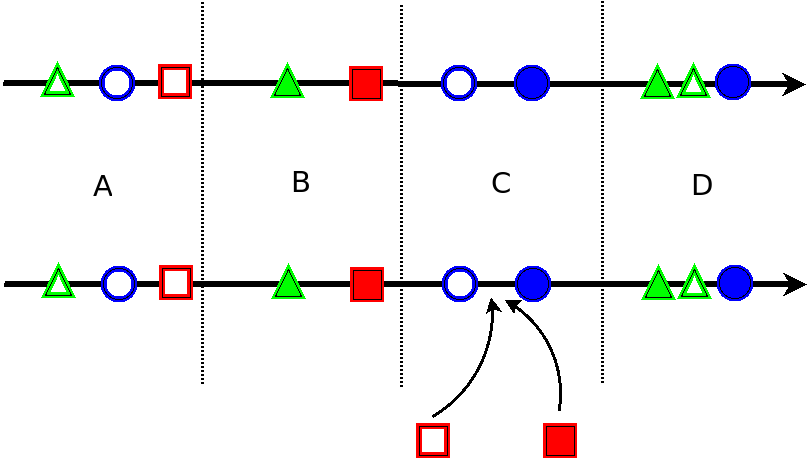
\includegraphics[scale=0.50]{figure/dc.png}
\caption[分而治之的计算策略示意图]{分而治之的计算策略示意图。实心符号表示产生算符,空
心符号表示表示消灭算符。不同的颜色与形状表示不同的轨道。图中展示的是往左起第三部分插入
一对算符的情况。}
\label{fig:dac}
\end{figure}

{\color{red}含义}:在广义相互作用版本的量子杂质模型求解器中,为了提高计算效率,通常将虚时
间轴$[0,\beta)$划分为npart个部份,分别计算每个部份的贡献。在随机产生新的图形时,首先
判断是那个部份上的算符发生了变化,然后再更新该部份的贡献。这就是所谓的"分而治之"的策
略(参见示意图\ref{fig:dac})。

{\color{green}类型}:integer

{\color{blue}缺省}:16

{\color{brown}组件}:仅{\begonia}与{\lavender}组件

{\color{purple}注解}:npart的取值十分讲究,如果取值过小,那么起不到加速的效果;如果取值过大,
那么计算开销也会随之增大。假定当前模型的能带数目为nband,平均的微扰展开阶数为$\langle k 
\rangle$,那么npart的最优取值应符合如下公式:

\begin{equation}
2\sqrt{3 \langle k\rangle \text{nband}} < \text{npart} < 4\sqrt{3 \langle k \rangle \text{nband}}
\end{equation}

\section{nflip }
\label{sec:nflip}

{\color{red}含义}:控制量子杂质模型求解器进行GLOBAL FLIP操作的频率。亦即每
隔nflip个Monte Carlo sampling进行一次GLOBAL FLIP操作。为了避免量子杂质模型
求解器在运行过程中陷入到某种非物理的有序态中,定期进行GLOBAL FLIP操作是十
分有必要的。在{\iqist}中,我们定义了三种基本的GLOBAL FLIP操作,用内部
整型变量cflip标示:
\begin{itemize}
\item cflip = 1,任意挑选两条对称性相同的轨道,对其上的量进行交换。 
\item cflip = 2,依次选择每条能带,交换其(名义上的)spin up和spin down的部分。
\item cflip = 3, 同时选择所有能带,各自交换其(名义上的)spin up和spin down的部分。
\end{itemize}
nflip也有三种取值可能:
\begin{itemize}
\item nflip = 0,GLOBAL FLIP的周期无限长,也就是不进行GLOBAL FLIP。
\item nflip > 0,组合cflip = 2和cflip = 3这两种GLOBAL FLIP模式,前者占80\%,后者占20\%。
\item nflip < 0,组合cflip = 1和cflip = 3这两种GLOBAL FLIP模式,前者占80\%,后者占20\%。
\end{itemize}

{\color{green}类型}:integer

{\color{blue}缺省}:2000

{\color{brown}组件}:全部

{\color{purple}注解}:如果需要考虑含自旋$-$轨道耦合的系统或者是系统具有
磁序,建议选择nflip = 0。

\section{ntherm}
\label{sec:ntherm}

{\color{red}含义}:在正式开始测量之间,需要进行thermalization,以使得系统达到
平衡。ntherm表示在达到平衡之间,需要进行的Monte Carlo sampling次数。

{\color{green}类型}:integer

{\color{blue}缺省}:200000

{\color{brown}组件}:全部

{\color{purple}注解}:ntherm一般不要超过nsweep的1/10。

\section{nsweep}
\label{sec:nsweep}

{\color{red}含义}:总的Monte Carlo sampling次数。

{\color{green}类型}:integer

{\color{blue}缺省}:20000000

{\color{brown}组件}:全部

{\color{purple}注解}:nsweep不能太小,太小无法保证测量精度。但是也不能太大,最
大不宜超过200000000。在data binning计算模式(isbin = 2,参见第\ref{sec:isbin}节)
中,nsweep和nwrite会自动增加为原来的十倍。如果nsweep的原始值太大,那么最终的
值会超出integer的数值范围,导致运行错误。

在并行运行模式中,假定采用nprocs个进程,那么每个进程都同样执行nsweep
个Monte Carlo sampling,而不是每个进程执行nsweep/nprocs个Monte Carlo sampling。因
此,如果用户采用大量处理器进行并行计算,那么可以适当减少nsweep的数值。但是
nsweep的最小取值不能小于ntherm,也不能小于nwrite,nmonte,与ncarlo中的任意
一个值。我们强烈建议nsweep的最小取值不要小于缺省值。

\section{nwrite}
\label{sec:nwrite}

{\color{red}含义}:输出中间结果的频率。亦即每间隔nwrite次Monte Carlo sampling,
量子杂质求解器会输出一些中间结果到文件中供用户分析,用户可依此判断计算结果是
否正确合理,如果不正确,那么可以及时终止任务,节约计算时间。目前主要输出的中
间结果主要有:$E_{\text{kin}}$,$E_{\text{pot}}$,$E_{\text{tot}}$,
$\langle S_{z} \rangle$,$G(\tau)$与histogram(亦即$P_{\text{H}}$)。

{\color{green}类型}:integer

{\color{blue}缺省}:2000000

{\color{brown}组件}:全部

{\color{purple}注解}:nwrite不宜太小,如果nwrite太小,这意味着频繁输出中间结果,
这样有两个坏处:(1)加重了IO的负担;(2)每次输出之前,各个并行进程之间要同步,通
信交换数据,会降低执行效率。

此外,在data binning模式中(isbin = 2),还利用nsweep与nwrite的比值来决定data bin
的数目。关于isbin参数的详情,请参阅第\ref{sec:isbin}节,关于nsweep参数的详情,
请参阅第\ref{sec:nwrite}节。

\section{nclean}
\label{sec:nclean}

{\color{red}含义}:量子杂质模型求解器进行clean update的频率。亦即每间
隔nclean次Monte Carlo sampling进行一次clean update,以保证合理的数值精度。

{\color{green}类型}:integer

{\color{blue}缺省}:100000

{\color{brown}组件}:全部

{\color{purple}注解}:每间隔nclean步,量子杂质模型求解器会根据当前的图形
配置从头计算$G(i\omega)$,以消除长期累积的数值误差。此参数一般无须改动。

\section{nmonte}
\label{sec:nmonte}

{\color{red}含义}:用于控制观测量的测量间隔。受影响的物理量有$G(i\omega)$, $E_{\text{tot}}$, 
$E_{\text{kin}}$, $E_{\text{pot}}$,$\langle S_{z} \rangle$,$\langle n_{i} \rangle$,
$\langle n_{i} n_{j} \rangle$,$\langle S_{z}(0)S_{z}(\tau)\rangle$,
$\langle N(0)N(\tau)\rangle$,$\chi(i\omega,i\omega^{\prime},\nu)$与
$\mathcal{F}(i\omega,i\omega^{\prime},\nu)$。

{\color{green}类型}:integer

{\color{blue}缺省}:10

{\color{brown}组件}:全部

{\color{purple}注解}:为了避免相邻两次测量之间产生关联,这两次测量之间需要间隔
nmonte个Monte Carlo sampling。nmonte不宜过大,过大会浪费抽样时间,也不宜过小,过
小则易产生关联。恰当的nmonte取值应满足以下关系:

nmonte * P$_{\text{insert}}$ $\ge$ 1

其中P$_{\text{insert}}$为INSERT KINK操作的接受概率,详情请参阅第\ref{sec:terminal}
节。如果用户的计算对上述物理量的精度要求不高,那么可以把nmonte设为一个很大的数值,
这样可以提高计算效率。

\section{ncarlo}
\label{sec:ncarlo}

{\color{red}含义}:用于控制观测量的测量间隔。受影响的物理量有$G(\tau)$,$F(\tau)$
与$P(\Gamma_i)$。

{\color{green}类型}:integer

{\color{blue}缺省}:10

{\color{brown}组件}:全部

{\color{purple}注解}:为了避免相邻两次测量之间产生关联,这两次测量之间需要间隔
ncarlo个Monte Carlo sampling。ncarlo不宜过大,过大会浪费抽样时间,也不宜过小,过
小则易产生关联。恰当的ncarlo取值应满足以下关系:

ncarlo * P$_{\text{insert}}$ $\ge$ 1

其中P$_{\text{insert}}$为INSERT KINK操作的接受概率,详情请参阅第\ref{sec:terminal}
节。如果用户的计算对$G(\tau)$,$F(\tau)$与$P(\Gamma_i)$的精度要求不高,那么可以
把ncarlo设为一个很大的数值,这样可以提高计算效率。
